\chapter{Testing and Results} \label{chap:testing_and_results}

In order to evaluate each of the networks implemented in the previous chapter, various tests were conducted. The main forms of evaluation were previously outlines in \cref{sec:evalutaion_metrics}, allowing for a comprehensive understanding of network performance. As well as this some explanation of the findings are also given.

\section{Data Pre-processing}

The data was converted to the z-score as described in \cref{ssec:data_preprocessing_design}, which made the network learn more stably and ensure any patterns found were more robust and easily applicable to unseen data. This effect was much more apparent on the reconstructed video sequences since the intensities tended to vary much more than the intensities from integrated frames. This is since the values from the integrated frames were naturally `centred' around similar values.

\section{Two-phase Intensity Reconstruction Models}

Most current classification networks are built to harness the features of video streams from frame-based cameras. To this end, networks were created to use these networks on intensity reconstructions from pre-built networks like E2VID (as described in \cref{ssec:video_reconstruction}). The results of such a network are given in this next section.

\subsection{Intensity Reconstruction}

The E2VID reconstruction network (as described in \cref{ssec:video_reconstruction}) was used to recreate intensity videos from events. It was evident that the reconstructions created were robust and relatively to to life. The reconstructions were not effected by adverse lighting effects or fast motions, which can be verified in \cref{fig:intensity_reconstructed_frames}, which shows a reconstruction of a video of a runner in a sunny environment. It is evident that even in sunny conditions the event camera is able to capture high contrast details such as buildings in the background against the sunlight. Now, modern computer vision techniques could still be applied to event data, while still preserving the many benefits the event model presents. It was interesting to note the performance of the reconstruction model on inputs with few moving parts. Since events are only triggered when there is an intensity change on any given pixel on the sensor, only regions with motion in them showed up as events, and the nature of all the space with no motion was not easily inferable. This can clearly be seen in \cref{fig:wave_in_lightings_reconstructions}, where only parts of the scene were accurately reconstructed. This did not, however, pose much of a problem for tasks such as gesture recognition, since the motion is exactly what is being classified, however for other tasks such as object recognition it had to be ensured that there was some sort of motion of either the object or the camera for the reconstruction algorithm to be effective.

\begin{figure}[htb]%
    \centering
    \subfloat[\centering]{{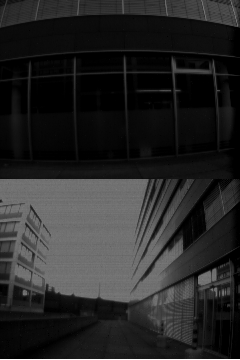
\includegraphics[width=0.25\textwidth]{testingandresults/images/outdoor_frames.png}}}%
    \qquad
    \subfloat[\centering]{{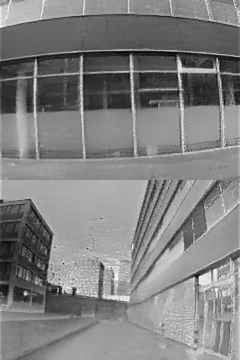
\includegraphics[width=0.25\textwidth]{testingandresults/images/outdoor_recontstructed_frames.png}}}%
    \caption{Figure showing matching video \textbf{(a)} and reconstructed frames \textbf{(b)} from the event camera dataset\cite{EventCameraDataset}.}%
    \label{fig:intensity_reconstructed_frames}%
\end{figure}

\Cref{fig:wave_in_lightings_reconstructions} shows that event-cameras do indeed allow for higher fidelity video capture in a wider range of lighting conditions that frame-based cameras (as explained in \cref{ssec:event_camera_benefits}). In all lighting conditions the video reconstruction was largely the same, since the events triggered were very similar in all cases. The logarithmic characteristics of the event-sensor pixels are the reason for this, since the thresholds for the triggering of events is not static. Since the reconstructions are consistent across lighting conditions, this also means that the reconstruction is more reliable, and the classification algorithm works better in adverse conditions in general \color{red} TODO: get figures and images to prove this \color{black}. The E2VID reconstruction uses fixed-size event windows. This means that each input has $ n $ events, and each input therefore has an equal amount of information. This way the output data can be of a high fidelity even with large amounts of motion. For example event though the motion of the hand is very large in this video, the individual fingers and details are still clearly visible in every frame.

\begin{figure}[htb]%
    \centering
    \subfloat[\centering]{{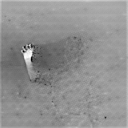
\includegraphics[width=0.18\textwidth]{testingandresults/images/dvs_wave_fluorescent_led.png}}}%
    \qquad
    \subfloat[\centering]{{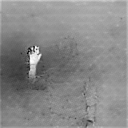
\includegraphics[width=0.18\textwidth]{testingandresults/images/dvs_wave_fluorescent.png}}}%
    \qquad
    \subfloat[\centering]{{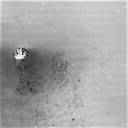
\includegraphics[width=0.18\textwidth]{testingandresults/images/dvs_wave_lab.png}}}%
    \qquad
    \subfloat[\centering]{{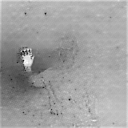
\includegraphics[width=0.18\textwidth]{testingandresults/images/dvs_wave_led.png}}}%
    \qquad
    \subfloat[\centering]{{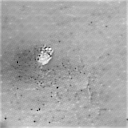
\includegraphics[width=0.18\textwidth]{testingandresults/images/dvs_wave_natural.png}}}%
    \caption{A waving motion being reconstructed from events captures by DVS128 event camera under different lighting conditions.The lighting conditions are as follows; \textbf{(a)} fluorescent led, \textbf{(b)} fluorescent, \textbf{(c)} lab lighting, \textbf{(d)} led lighting and \textbf{(e)} natural lighting.}%
    \label{fig:wave_in_lightings_reconstructions}%
\end{figure}

However, the quality of the reconstructions was not as impressive for datasets where the input is vastly different to the data E2VID was trained on (see \cref{fig:nmnist_reconstructions}). For example, with the NMNIST dataset\cite{NMNIST}, the input size was very small. This was a deliberate choice so that the format of NMNISt closely matches the format of MNIST, allowing for efficient training and testing of networks. However, the reconstruction of these samples was very rudimental, showing results similar to an edge map rather than a full reconstruction. This is one of the factors that made the two-phase pipeline less effective for this dataset as compared to the DVS128 Gesture reconstructions. This disparity could be eliminated if E2VID was re-trained on the specific data that was input, however for this project such datasets were not readily available, nor the time to train the network.

\begin{figure}[htb]%
    \centering
    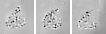
\includegraphics[width=0.6\textwidth]{testingandresults/images/nmnist_reconstructions.png}
    \caption{A figure showing three reconstructed frames from a recording of the MNIST character `6'.}%
    \label{fig:nmnist_reconstructions}%
\end{figure}

\subsubsection{Classification Results}

The confusion matrices for the classification of the intensity reconstructed NMNIST dataset can be seen in \cref{fig:nmnist_recon_c_matrices}. It is clear that the performance of the network is worse on more challenging characters such as 6, 8 and 9. This is understandable, considering the corresponding reconstructions of these classes is of noticeable poorer quality (see \cref{fig:nmnist_reconstructions}). Although the reconstructions are sometimes distinguishable by eye, the lines are often blurred. Due to the small scale of the dataset the resulting video stream is also of a small size, meaning less details can could be represented in the relatively low resolution images.

For the 3D convolutional neural network, the precision was often lower for these difficult classes. This means that these classes were over-represented in the predictions, when it should have been the other classes being detected (i.e., false positives). The purely convolutional network was able to identify patterns in the data due to its large number of trainable parameters, however this also meant that it over-trained on the features present in the more complex classes, often finding them in samples of the other classes.

Interestingly, with the LSTM networks it is instead the recall that was lower for these challenging classes, meaning many of the samples of these classes were misclassified (false negatives). The cause for this may be that the had fewer trainable parameters, but the recurrent capabilities made up for this allowing for the network to learn temporal patterns more reliably.

Overall the f1 measure acts as a balanced measure between precision and recall, since the data is not biased to any one class. The f1 score is superior for the 3D convolutional network and custom convolutional network, which both have similar performance on the test dataset. This makes sense since the temporal patterns are less important in the case of number classification, since motion is not prevalent or interesting.

\begin{figure}[htb]%
    \centering
    \subfloat[\centering]{{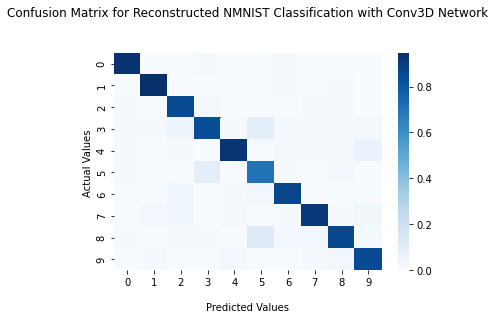
\includegraphics[width=0.4\textwidth]{testingandresults/images/c_matrix_nmnist_recon_conv3d.png}}}%
    \qquad
    \subfloat[\centering]{{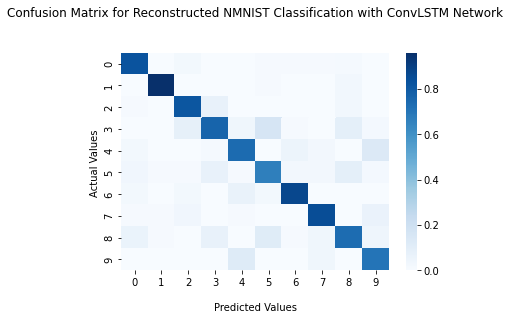
\includegraphics[width=0.4\textwidth]{testingandresults/images/c_matrix_nmnist_recon_convlstm.png}}}%
    \qquad
    \subfloat[\centering]{{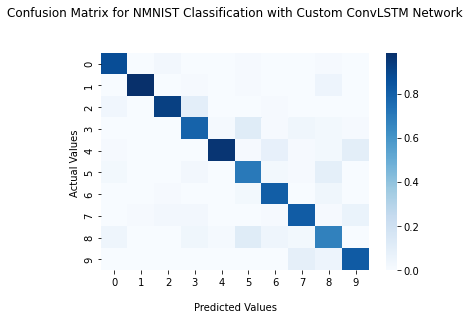
\includegraphics[width=0.4\textwidth]{testingandresults/images/c_matrix_nmnist_recon_custom_convlstm.png}}}%
    \caption{Confusion matrices for intensity reconstructed NMNIST classification with various networks; \textbf{(a)} conv3D, \textbf{(b)} convLSTM, \textbf{(c)} custom convLSTM.}%
    \label{fig:nmnist_recon_c_matrices}%
\end{figure}

\Cref{tab:conv3d_nmnist_recon_evaluation_metrics}, \cref{tab:conv_lstm_nmnist_recon_evaluation_metrics}, and \cref{tab:custom_conv_lstm_nmnist_recon_evaluation_metrics} show the performance evaluation of each of the networks on the intensity reconstructed NMNIST dataset in more detail.

\vspace{10pt}

The confusion matrices for the classification of the intensity reconstructed DVS128 Gesture dataset can be seen in \cref{fig:dvs128_recon_c_matrices}. Here the findings were a little different than for the NMNIST dataset. Firstly, it is important to note that when attempting to reconstruct the videos and pass them into each of the networks, the amount of memory often became an issue. This in itself is a clear indication of a large difference between the event and frame representations. After conversion, the frame-based video was of a much larger size and density than the event streams it was created from. In other words the efficiency of encoding was much higher in the case of event streams than intensity videos. For this reason it was not even feasible to run the ConvLSTM network with this data since both the memory and time requirements were much too high.

Between the purely convolutional and LSTM network there were still many interesting conclusions to be drawn. Th performance disparity between the two was of a much larger scale than with the reconstructed NMNIST dataset. The reason for this is that the recurrent neural network was much better at recognising temporal patters as well as spatial ones in the data, which is much more important in the case of gesture recognition. For this reason the overall accuracy was much better with the LSTM network. For cases with very similar frames (such as clockwise and counter-clockwise arm rotations), the LSTM had far better precision as well.

\begin{figure}[htb]%
    \centering
    \subfloat[\centering]{{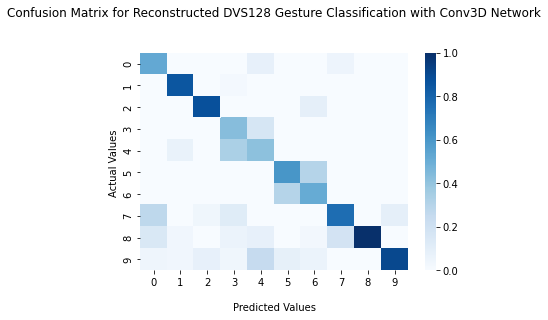
\includegraphics[width=0.4\textwidth]{testingandresults/images/c_matrix_dvs128_recon_conv3d.png}}}%
    \qquad
    \subfloat[\centering]{{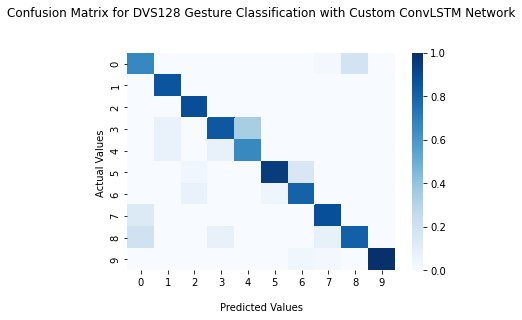
\includegraphics[width=0.4\textwidth]{testingandresults/images/c_matrix_dvs128_recon_custom_convlstm.png}}}%
    \caption{Confusion matrices for intensity reconstructed  DVS128 Gesure classification with various networks; \textbf{(a)} conv3D, \textbf{(b)} custom convLSTM.}%
    \label{fig:dvs128_recon_c_matrices}%
\end{figure}

\Cref{tab:conv3d_dvs128_recon_evaluation_metrics} and \cref{tab:custom_conv_lstm_dvs128_recon_evaluation_metrics} show the performance evaluation of each of the networks on the intensity reconstructed DVS128 Gesture dataset in more detail. 

\section{End-to-end Event Classification Models}

The benefits of the event driven camera (as described in \cref{ssec:event_camera_benefits}) were evident in the acquired results. As opposed to tradition frame-based cameras, high frequency data is not lost when processing events. There are spikes for every event at a much more granular scale in the temporal dimension in the event camera when compared to the frame camera, meaning fast movements were captured more reliably since events are captured at the $\mu s$ scale, no longer restricted by the frame-rates of modern cameras (which often results in motion blur).

\subsection{Frame Integration}

It is evident that modern computer vision techniques have been developed with frame-based cameras in mind, and so modern networks achieve good accuracy, and are able to find patterns well, on frame-based data. For this reason the common technique of integrating frames\cref{ssec:frame_integration} results in regular frames, akin to the ones a regular camera generates, in order to feed into such networks. It does, however, still pose many benefits when compared to the frames from a regular camera. As mentioned previously information between frames is still not lost or degraded since the events are still captured and visible in each frame. As well as this, the frames generated from events inherently focussed on the points of interest in the image, since these were the only ones in motion in the frame. Most common architectures (such as the one proposed by Raimundo F. Pinto \textit{et al.} for static hand gesture recognition\cite{StaticHandGesture}) for classical videos feature an intermediate layer to remove backgrounds and other noise from images from the image to focus on the points of interest. In this way the intermediate layer could be omitted when operating on the integrated event frames, since the output was already similar to an edge map. It is conceivable, however, that in noisy environments with lots of motion this stage would still be necessary.

It was also interesting to note the inherent ability of neuromorphic cameras to capture points of interest. When using the frame integration method, the result was very similar to an edge map, which is often the primary step of image analysis using convolutional neural networks to images in existing networks already. \Cref{fig:canny_edge_detection_nmnist} shows the effect of carrying out canny edge detection\cite{CannyEdgeDetection} on an integrated frame from the NMNIST dataset. The sample is taken from a recording of the number `0', and it can be seen that the original frame is in essence just a noisy edge map of the number. The steps taken for canny edge detection were as follows;

\begin{enumerate}
    \item Smooth image by convolving with an averaging filter of the form: $ \begin{bmatrix}
        \frac{1}{4^2} & \frac{1}{4^2}  & \frac{1}{4^2}  & \frac{1}{4^2} \\
        \frac{1}{4^2} & \frac{1}{4^2}  & \frac{1}{4^2}  & \frac{1}{4^2} \\
        \frac{1}{4^2} & \frac{1}{4^2}  & \frac{1}{4^2}  & \frac{1}{4^2} \\
        \frac{1}{4^2} & \frac{1}{4^2}  & \frac{1}{4^2}  & \frac{1}{4^2} \\
    \end{bmatrix} $
    \item Sobel edge detection was carried out in order to find the edges of the smoothed image. To do this the image was convolved with the following matrices: $ S_x =
    \begin{bmatrix}
        -1 & 0 & 1 \\
        -2 & 0 & 2 \\
        -1 & 0 & 1 \\
    \end{bmatrix} $ and $ S_y = 
    \begin{bmatrix}
        1 & 2 & 1 \\
        0 & 0 & 0 \\
        -1 & -2 & -1 \\
    \end{bmatrix} $. These matrices got the pixel gradients in the x and y directions, and taking their magnitudes ( $ \sqrt{S_x^2 + S_y^2} $ ) gives the edges map of the frame.
    \item Hysteresis thresholding allowed for weaker edges to be counted as long as they are connected to stronger ones. Then non-maximum suppression was applied to get a single line for every edge (by finding the strongest point of every line in the direction of its gradient).
\end{enumerate}

This refined edge map could have been part of the pre-processing of the data before being passed into the network, but it was found that this was not beneficial to network training. This was because some information is lost in the smoothing process, and any feature mapping was done efficiently during the training of convolutional networks anyway.

\begin{figure}[htb]%
    \centering
    \subfloat[\centering]{{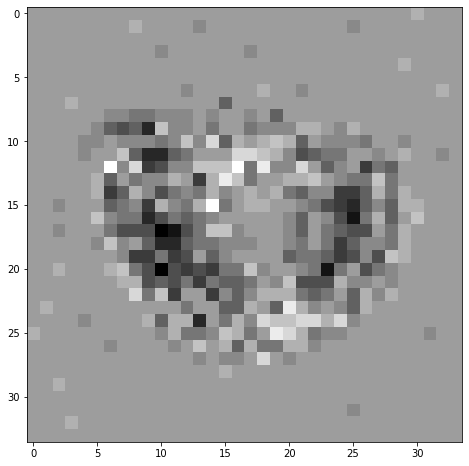
\includegraphics[width=0.18\textwidth]{testingandresults/images/denoise_origional.png}}}%
    \qquad
    \subfloat[\centering]{{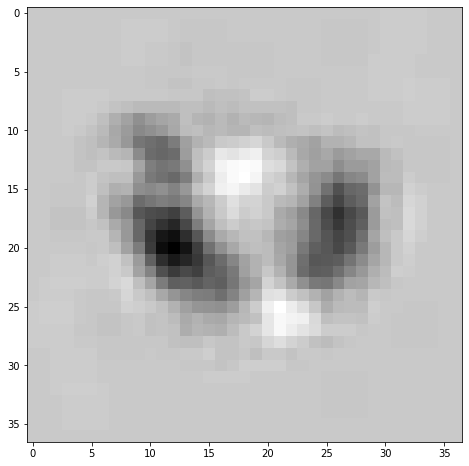
\includegraphics[width=0.18\textwidth]{testingandresults/images/denoise_smoothed.png}}}%
    \qquad
    \subfloat[\centering]{{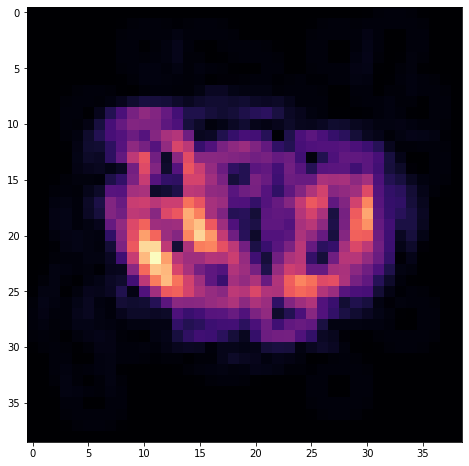
\includegraphics[width=0.18\textwidth]{testingandresults/images/denoise_edge_map.png}}}%
    \qquad
    \subfloat[\centering]{{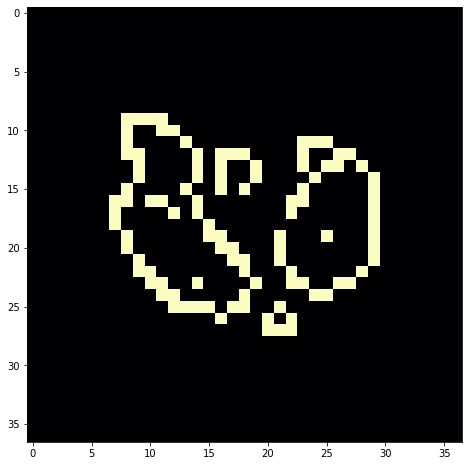
\includegraphics[width=0.18\textwidth]{testingandresults/images/denoise_hysteresis.png}}}%
    \caption{Progression of canny edge detection on integrated frame of a sample from the NMNIST dataset with class `0'. The steps are as follows; \textbf{(a)} original integrated frame, \textbf{(b)} smoothed, \textbf{(c)} edge detection, and \textbf{(d)} Non-maximum suppression and hysteresis thresholding.}%
    \label{fig:canny_edge_detection_nmnist}%
\end{figure}

\subsubsection{Classification Results}

The confusion matrices for the classification of the frame-integrated  NMNIST dataset can be seen in \cref{fig:nmnist_c_matrices}. In terms of precision of classification, all networks perform relatively well. However, the 3D convolutional network and the custom convolutional LSTM network were marginally more effective, achieving a higher accuracy and correctly classifying more challenging event streams. Where this is most apparent is when classifying numbers such as 3, since with the base convolutional LSTM network these were sometime misclassified as an 8 or 9.

The performance of each network on the frame integrated NMNIST was better overall than with the frame integrated equivalent (as is evident by the superior f-score of the classification networks), which may be due to the fact that temporal information was not lost, as was the case in the reconstructed video stream. Due to the poor performance of the intensity reconstructions overall, it was outperformed in most, if not all cases.

\begin{figure}[htb]%
    \centering
    \subfloat[\centering]{{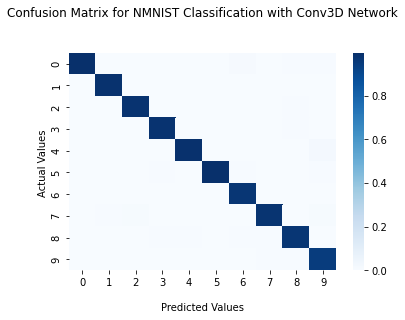
\includegraphics[width=0.4\textwidth]{testingandresults/images/c_matrix_nmnist_conv3d.png}}}%
    \qquad
    \subfloat[\centering]{{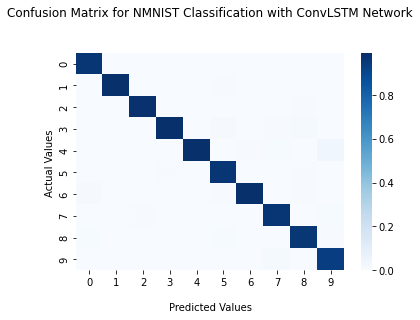
\includegraphics[width=0.4\textwidth]{testingandresults/images/c_matrix_nmnist_convlstm.png}}}%
    \qquad
    \subfloat[\centering]{{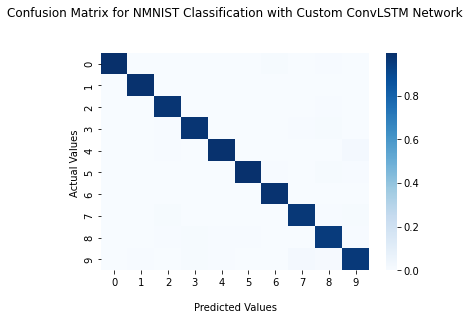
\includegraphics[width=0.4\textwidth]{testingandresults/images/c_matrix_nmnist_custom_convlstm.png}}}%
    \caption{Confusion matrices for frame-integrated NMNIST classification with various networks; \textbf{(a)} conv3D, \textbf{(b)} convLSTM, \textbf{(c)} custom convLSTM.}%
    \label{fig:nmnist_c_matrices}%
\end{figure}

\Cref{tab:conv3d_nmnist_evaluation_metrics}, \cref{tab:conv_lstm_nmnist_evaluation_metrics}, and \cref{tab:custom_conv_lstm_nmnist_evaluation_metrics} show the performance evaluation of each of the networks on the frame-integrated NMNIST dataset in more detail. Once again the network has trouble classifying the difficult classes. We can see that the performance suffers more when compared to the networks analysing the integrated frames. Especially in the NMNIST dataset the edges are very significant for distinguishing between each class, which integrated frames excel at highlighting. The additional intensities added to the frames by E2VID seem to only hinder performance.

\vspace{10pt}

The confusion matrices for the classification of the frame-integrated DVS128 Gesture dataset can be seen in \cref{fig:dvs128_c_matrices}. The variance in performance between the networks is more apparent in this dataset than for the NMNIST dataset. The reason for this is that not only is object detection (of the human body) being undertaken by the system, but also action recognition across frames. It is evident that actions 4 and 5 (right arm clockwise and right arm counter-clockwise), as well as actions 6 and 7 (left arm clockwise and left arm counter-clockwise), were often misclassified as one another. The reason for this was that with length 20 frame integrated videos the fast rotational movement results in frames that look very similar in both directions \color{red} TODO: Maybe try to get some pictures to prove this \color{black}. This could be remedied by having more than 20 frames for each integrated video sequence. Other mistakes were more often made with the 3D convolutional network. For example 10 (air guitar) was quite often predicted for cases of classes 8 and 9 (air roll and air drums). 

\begin{figure}[htb]%
    \centering
    \subfloat[\centering]{{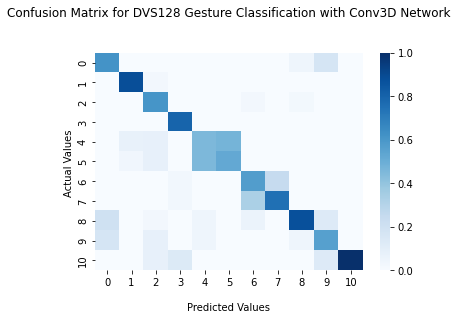
\includegraphics[width=0.4\textwidth]{testingandresults/images/c_matrix_dvs128_conv3d.png}}}%
    \qquad
    \subfloat[\centering]{{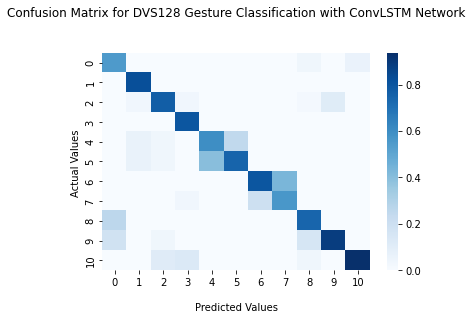
\includegraphics[width=0.4\textwidth]{testingandresults/images/c_matrix_dvs128_convlstm.png}}}%
    \qquad
    \subfloat[\centering]{{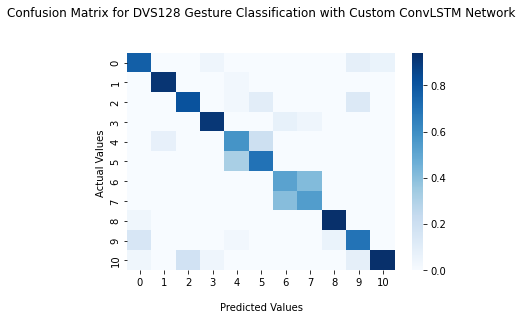
\includegraphics[width=0.4\textwidth]{testingandresults/images/c_matrix_dvs128_custom_convlstm.png}}}%
    \caption{Confusion matrices for frame-integrated  DVS128 Gesure classification with various networks; \textbf{(a)} conv3D, \textbf{(b)} convLSTM, \textbf{(c)} custom convLSTM.}%
    \label{fig:dvs128_c_matrices}%
\end{figure}

\Cref{tab:conv3d_dvs128_evaluation_metrics}, \cref{tab:conv_lstm_dvs128_evaluation_metrics}, and \cref{tab:custom_conv_lstm_dvs128_evaluation_metrics} show the performance evaluation of each of the networks on the frame-integrated DVS128 Gesture dataset in more detail.

\subsection{Custom Frame Integration}

Some tests were undertaken using the custom frame integration technique on the DVS128 Gesture dataset. As you can see, information can be stored to the same, or even smaller, temporal resolution in a lower channel image. \cref{fig:frame_integration_comparison} shows the left arm clockwise hand rotation gesture represented using the two techniques. In the interest of time, for the following testing the regular frame integration technique was used, since it is adequate for the sake of comparison. It is clear that the encoding is more efficient, since only single-channelled greyscale images are required with the custom integration method, and more fine-grained temporal information is retained since the intensity of the pixels signifies the amount of events occurring in any given pixel. For example, in the figure it is possible to visually know where the position of the arm is, as well as the movement it was going through, with the custom frame frame integration even without having to create too many individual integrated frames. We can see that when 20 integrated frames were created for the NMNIST dataset with the classical method, the motion is visible in one large blur, with no clear indication of the position of the arm for example.

\begin{figure}[htb]%
    \centering
    \subfloat[\centering]{{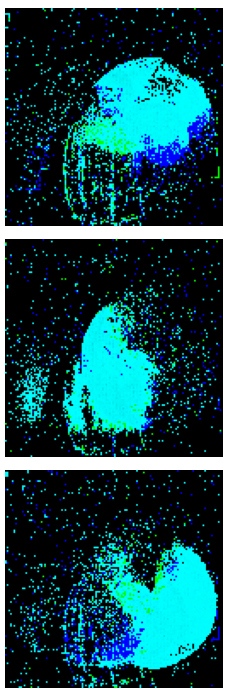
\includegraphics[width=0.18\textwidth]{testingandresults/images/classic_frame_integration.png}}}%
    \qquad
    \subfloat[\centering]{{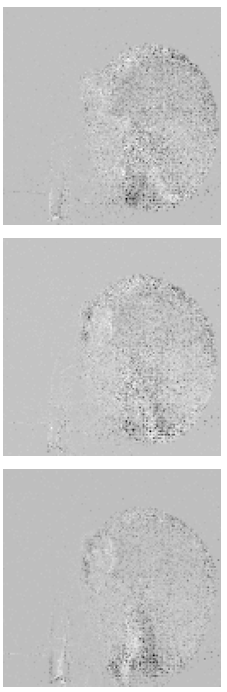
\includegraphics[width=0.18\textwidth]{testingandresults/images/custom_frame_integration.png}}}%
    \caption{Frame integration of arm rotation gesture from DVS128 Gesture dataset with two different methods; \textbf{(a)} classic frame integration, and \textbf{(b)} custom frame integration.}%
    \label{fig:frame_integration_comparison}%
\end{figure}

\color{red} TODO: Write some experiments for comparison of the two techniques. \color{black} 

\subsubsection{Clssification Results}

The confusion matrices for the classification of the frame-integrated  NMNIST dataset with the custom frame integration method can be seen in \cref{fig:nmnist_custom_frame_c_matrices}. \color{red} TODO: Write more about this and redo confusion matrices \color{black}.

\begin{figure}[htb]%
    \centering
    \subfloat[\centering]{{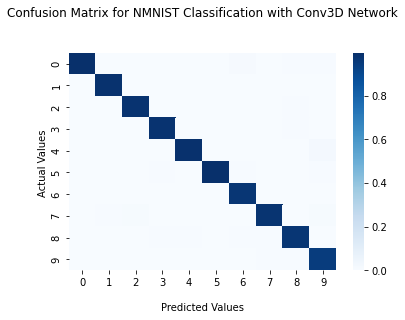
\includegraphics[width=0.4\textwidth]{testingandresults/images/c_matrix_nmnist_custom_frame_conv3d.png}}}%
    \qquad
    \subfloat[\centering]{{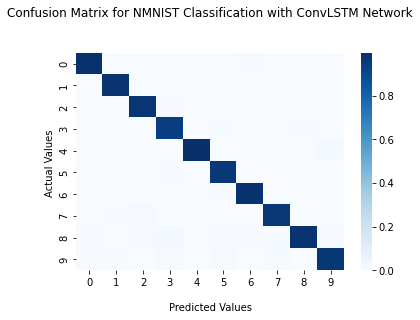
\includegraphics[width=0.4\textwidth]{testingandresults/images/c_matrix_nmnist_custom_frame_convlstm.png}}}%
    \qquad
    \subfloat[\centering]{{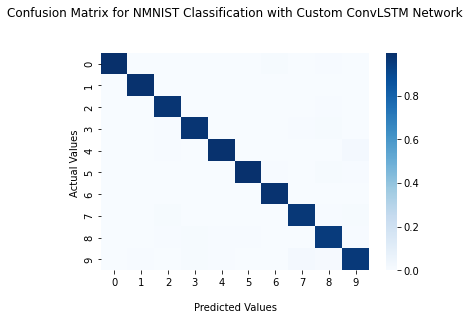
\includegraphics[width=0.4\textwidth]{testingandresults/images/c_matrix_nmnist_custom_frame_custom_convlstm.png}}}%
    \caption{Confusion matrices for custom frame-integrated NMNIST classification with various networks; \textbf{(a)} conv3D, \textbf{(b)} convLSTM, \textbf{(c)} custom convLSTM.}%
    \label{fig:nmnist_custom_frame_c_matrices}%
\end{figure}

\Cref{tab:conv3d_nmnist_custom_frame_evaluation_metrics}, \cref{tab:conv_lstm_nmnist_custom_frame_evaluation_metrics}, and \cref{tab:custom_conv_lstm_nmnist_custom_frame_evaluation_metrics} show the performance evaluation of each of the networks on the custom frame-integrated NMNIST dataset in more detail.

\color{red} TODO: Get result for custom frame-integrated DVS128 Gesture. \color{black}

\section{Network Comparisons}

% \begin{table}[htb]
%     \centering
%     \begin{tabular}{|| c | c | c ||}
%         \hline
%         Network     & NMNIST & DVS128 Gesture \\
%         \hline \hline
%         Conv3D Reconstruction Classifier           & 86.67\%    &   63.26\%    \\
%         \hline
%         Conv2D LTSM Reconstruction Classifier          & 79.60\%   &  -    \\
%         \hline
%         Custom LTSM Reconstruction Classifier         & 83.20\%  &   82.95\%   \\
%         \hline
%         Conv3D Frame Integration Classifier          &  98.74\%  &   69.44\%    \\
%         \hline
%         Conv2D LTSM Frame Integration Classifier         &  97.64\%  &    71.53\%    \\
%         \hline
%         Custom LTSM Frame Integration Classifier         &  97.70\% &   76.39\%     \\
%         \hline
%         Conv3D Custom Frame Integration Classifier          & 98.22\%   &      \\
%         \hline
%         Conv2D LTSM Custom Frame Integration Classifier         & 97.48\%   &  \\
%         \hline
%         Custom LTSM Custom Frame Integration Classifier         & 97.88\%  &        \\
%         \hline
%     \end{tabular}
%     \caption{A table showing classification accuracies of various models.}
%     \label{tab:network_performances_old}
% \end{table}

\begin{table}[htb]
    \centering
    \begin{tabular}{|| c | l | c | c | c ||}
        \hline
        \multicolumn{2}{|| c |}{Dataset} & Conv3D & ConvLSTM & Custom ConvLSTM \\
        \hline \hline
        \multirow{3}{*}{NMNIST} & Intensity Reconstructed & 86.67\% & 79.60\% & 83.20\%\\
        \cline{2-5}
         & Frame Integrated & 98.74\% & 97.64\% & 97.70\% \\
        \cline{2-5}
        & Custom Frame Integrated & 98.22\% & 97.48\% & 97.88\% \\
        \hline
        \multirow{3}{*}{DVS128 Gesture} & Intensity Reconstructed & 63.26\% & - & 82.95\% \\
        \cline{2-5}
         & Frame Integrated & 69.44\% & 71.53\% & 76.39\% \\
        \cline{2-5}
         & Custom Frame Integrated & & & \\
        \hline
    \end{tabular}
    \caption{A table showing classification accuracies of various models.}
    \label{tab:network_performances}
\end{table}

The full table of classification accuracies can be seen in \cref{tab:network_performances}. Here, the different strengths of the various networks becomes apparent in this comparison. For the simple object classification task on the NMNIST dataset, the higher capacity 3D convolutional network outperformed the others. However, in the more complex task of gesture recognition on the DVS128 Gesture dataset it struggled. The reason for this is that though it is excellent at detecting spacial patterns in each frame, it is less able to detect the temporal patterns prevalent in the gestures.

% \begin{table}[htb]
%     \centering
%     \begin{tabular}{|| c | c | c ||}
%         \hline
%         Network     & NMNIST & DVS128 Gesture \\
%         \hline \hline
%         Conv3D Reconstruction Classifier        &  0h05m02s    &    1h09m43s  \\
%         \hline
%         Conv2D LTSM Reconstruction Classifier        &  0h14m28s    &   -   \\
%         \hline
%         Custom Conv2D LTSM Reconstruction Classifier         &  0h03m26s \color{red} why so short \color{black}  &    3h13m45s   \\
%         \hline
%         Conv3D Frame Integration Classifier          &  0h17m20s  &   0h34m49s    \\
%         \hline
%         Conv2D LTSM Frame Integration Classifier         & 0h42m02s  &    0h08m33s    \\
%         \hline
%         Custom LTSM Frame Integration Classifier         & 0h10m50s   &    \color{red} 1h24m19s \color{black}    \\
%         \hline
%         Conv3D Custom Frame Integration Classifier          & 1h43m03s   &       \\
%         \hline
%         Conv2D Custom LTSM Frame Integration Classifier         & 1h03m09s   &       \\
%         \hline
%         Custom LTSM Custom Frame Integration Classifier         &  1h12m10s  &        \\
%         \hline
%     \end{tabular}
%     \caption{A table showing training times various models.}
%     \label{tab:network_training_times}
% \end{table}

\begin{figure}[htb]
    \centering
    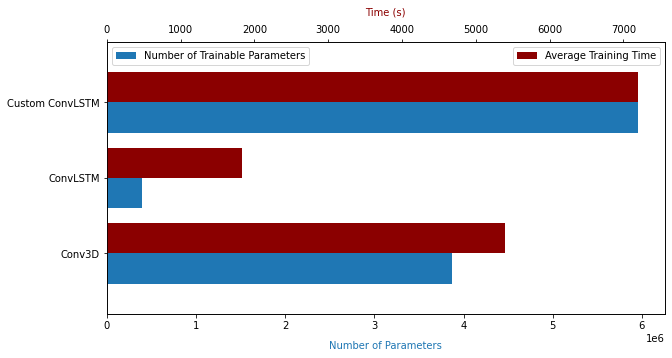
\includegraphics[width=0.8\textwidth]{testingandresults/images/training_time_and_trainable_parameters.png}
    \caption{A figure showing the training times and number of trainable parameters of each network.}
    \label{fig:training_times_and_trainable_parameters}
\end{figure}

The training times for each of the networks on the datasets can be seen in \cref{fig:training_times_and_trainable_parameters}. It is evident that the networks with a higher capacity had higher training times. The 3D convolution network in particular had much longer training times than the other two networks, since it had many more parameters to optimise via back-propagation. It should be noted that for the networks in missing classification accuracies in \cref{tab:network_performances} the system often encountered an Out Of Memory (OOM) error when attempting create a tensor of larger batch size. For these cases a smaller batch size was used, resulting in slightly higher training times, as well as possible skewed results. If even this was not sufficient, results were not taken for these cases.

\subsection{3D Convolutional Networks vs Recurrent Networks}

The drawback to the 3D convolutional network is that the number of trainable parameters (as can be seen in \cref{ssec:conv_3d_network_design}) is much higher than the other networks, and so the training and inference times were considerably higher than the other networks as well (as can be seen in \cref{fig:training_times_and_trainable_parameters}).

\subsection{Spiking Neural Networks}

\subsubsection{Converted 3D Convolutional Network}

As mentioned in \cref{sssec:firing_rate_scaling}, there is a compromise to be made when attempting to scale neuron firing rates to get a better accuracy. When firing rates are scaled past a certain level, the network becomes equivalent to a non-spiking network. This would mean the loss of the benefits of sparse encoding the the SNN. The effect of over-scaling firing rate can be seen in \cref{fig:over_scaling_firing_rate}, where a very high firing rate results in a network very similar to a non-spiking neural network.

\begin{figure}[htb]%
    \centering
    \subfloat[\centering]{{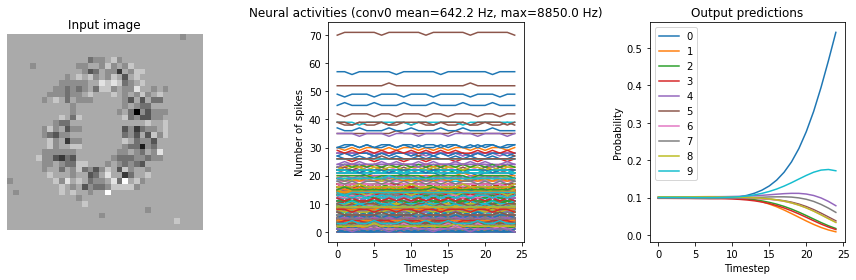
\includegraphics[width=0.7\textwidth]{testingandresults/images/overscaled_firing_rate.png}}}%
    \qquad
    \subfloat[\centering]{{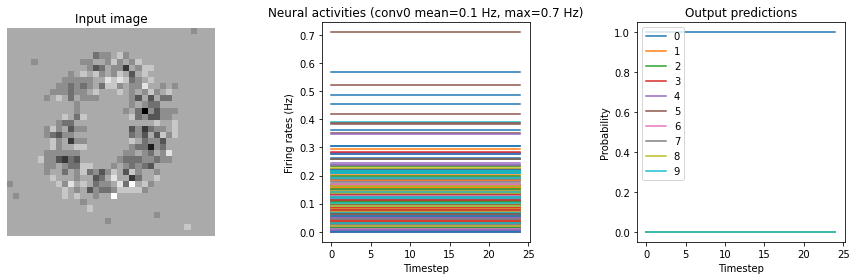
\includegraphics[width=0.7\textwidth]{testingandresults/images/non_spiking_comparison.png}}}%
    \caption{Comparison of spiking neural network with firing rate over-scaled \textbf{(a)} and a the equivalent non-spiking neural network \textbf{(b)}.}%
    \label{fig:over_scaling_firing_rate}%
\end{figure}

The relationship between firing rates and performance can be seen in \cref{fig:spiking_perfromace_with_varying_spike_rate}, where the accuracy gets closer to the non-spiking network as the spiking rate is artificially inflated to infinity. It was found that for the conv3D network, comparable performance could be obtained while keeping the data-flow through each network quite sparse, since close to 100\% relative performance could be reached with an average neuron spiking rate of less than 1Hz for both the NMNIST and DVS128 datasets. Especially for the DVS128 dataset, with very few average neuron spikes, the network achieved good relative performance.

\begin{figure}[htb]
    \centering
    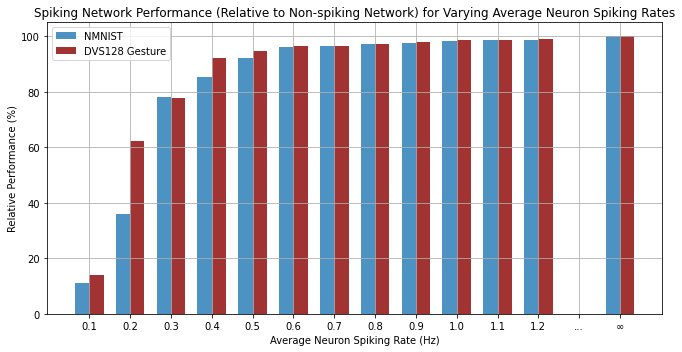
\includegraphics[width=0.8\textwidth]{testingandresults/images/spiking_perfromace_with_varying_spike_rate.png}
    \caption{A figure showing the performance of the spiking 3D conv network relative to its non-spiking equivalent with varying spike rates.}
    \label{fig:spiking_perfromace_with_varying_spike_rate}
\end{figure}

\subsubsection{Legendre Memory Unit Network}

\begin{table}[htb]
    \centering
    \begin{tabular}{|| c | c | c ||}
        \hline
        Network     & NMNIST & DVS128 Gesture \\
        \hline \hline
        Non-spiking LMU        &  90.2\%    &    60\%  \\
        \hline
        Spiking LMU        &  60\%    &      \\
        \hline
    \end{tabular}
    \caption{A table showing the performance of LMU networks on various datasets.}
    \label{tab:lmu_performance}
\end{table}

\cref{tab:lmu_performance} shows the promise of LMUs as a recurrent module for spiking neural networks. The performance before SNN conversion is similar to LSTM networks, and could feasibly improved with convolutional elements as was done with the convLSTM layer.

\color{red} TODO: Write about difficulties with spiking LSTM and experiments with LMU network. \color{black}